\documentclass[12pt]{article}
\usepackage{amsmath,amssymb,amsthm,bm}
\usepackage[usenames,dvipsnames]{xcolor}
\usepackage{graphicx}
%\usepackage{lmodern}
\usepackage[T1]{fontenc}
%\usepackage{textcomp}
\usepackage{pxfonts}
\usepackage{enumerate,verbatim,cite}
\usepackage[margin=1in]{geometry}
\usepackage{indentfirst}
%\usepackage{../../tex/pythonhighlight} %https://github.com/olivierverdier/python-latex-highlighting

\usepackage{fancyhdr}
\pagestyle{fancy}
%\addtolength{\headheight}{\baselineskip}
\addtolength{\footskip}{\baselineskip}
\renewcommand{\headrulewidth}{0pt}
\renewcommand{\footrulewidth}{0.4pt}
\fancyhf{}
\fancyfoot[L]{\textit{Last Modified: \today}}
\fancyfoot[C]{\thepage}


\usepackage[pdftex,bookmarks,hyperfigures,colorlinks
						,urlcolor=blue
						,citecolor=blue
						,linkcolor=blue
						,pdfstartview=FitH]{hyperref}


%\usepackage{epsf}
% \topmargin -0.5in \setlength{\textwidth}{6.in}
% \setlength{\textheight}{8.5in}
%\setlength{\evensidemargin}{0.25in}
% \setlength{\oddsidemargin}{0.25in}
\renewcommand{\r}{{\bf r}}
\newcommand{\dery}{\frac{dx}{dt}}
\renewcommand{\k}{{\bf k}}
\newcommand{\be}{\begin{equation}}
\newcommand{\ee}{\end{equation}}
%\usepackage[usenames,dvipsnames]{xcolor}
%\usepackage{hyperref}

\newcommand{\myTitleBox}{
\noindent\makebox[\linewidth][c]{%
  %
    \parbox{\paperwidth}{%
      \hspace*{\dimexpr\hoffset+\oddsidemargin+1in\relax}%
      \begin{minipage}{\dimexpr\textwidth-2\fboxsep-2\fboxrule\relax}
      {\large\textbf{\courseTitleS}\courseTitle\hfill}\vspace{2mm}\\
%      {\large\textbf{\topicsCoveredS}\topicsCovered\hfill}\vspace{2mm}\\
      {\large\courseInstructors\hfill}\vspace{2mm}\\
%      \secAuthor\hfill\sectionTimesV\\
%      \authorContact\hfill\sectionTime\\
      \end{minipage}
    %
  }%
}
}


\newcommand{\courseTitleS}{CS109B/STAT121B/APCOMP209a/CSCI109B}
\newcommand{\courseTitle}{ Advanced Topics in Data Science}
\newcommand{\courseInstructors}{\textbf{Instructors:} Mark Glickman, Pavlos Protopapas}
%\newcommand{\sectionTimesV}{Section Times}
%\newcommand{\sectionTime}{ Wed 3-4pm \& Wed 5:30-6:30 \& Thurs 2:30-3:30}
%\newcommand{\topicsCoveredS}{Advanced Section 6:}
%\newcommand{\topicsCovered}{ Topics in Supervised Classification}
%\newcommand{\authorContact}{nhoernle@g.harvard.edu}
%\newcommand{\secAuthor}{Nick Hoernle}
\newcommand{\emptyS}{ }

%\title{\textbf{CS 109A Final Project} \\ \bigskip \large{Urban Crime Prediction}}
\date{}

\begin{document}
%\myTitleBox

\noindent {\small{\sc{CS 109B/Stat 121B/AC 209B/CSCI 109B: Final Project} \hfill \\ \small{\sc{Glickman, Protopapas}} \hfill \\ 
\small{\sc{Dor Baruch, Michaela Kane, David Loving, \& Brandon Walker}}}
\begin{center}
\section*{Cancer Diagnosis in Medical Imaging}
\end{center}

%\maketitle

\subsection*{Problem Statement}

In the treatment and prevention of cancer, early detection plays a crucial and often life-saving role. One of the most common methods of early cancer detection is the CT (computer tomography) scan, which is used to detect anomalies in the form of pre-cancerous or cancerous nodules in body tissue. Human radiologists then study these scans and assess the severity and danger of any irregularities they observe.

However, the detection of nodules and their correct diagnosis is extremely challenging, as pre-cancerous nodules are often small, and even when they are visible, they often look like surrounding benign tissue formations [\ref{bib:baker}]. In an attempt to assist radiologists, recent years have seen the development and use of neural networks to help classify CT scans and other medical images for the sake of more accurate, early diagnosis and cancer prevention.

These networks are not infallible themselves, unfortunately, and there are instances in which humans place too much confidence in artificial intelligence without enough critical thought [\ref{bib:finale}]. As a result, there is an increasing demand for networks with a degree of explainability. If researchers and physicians can gain a better understanding of how a network makes its decisions, or what changes to the input variables have on the network's output, then it would be easier for them to accept the network's diagnosis. In the end, this makes for faster, more accurate assessments.  

For this project, we attempted to address this issue of explainability through the combination of visualization and Bayesian methods. First, we trained a U-Net on CT Scans from LUng Nodule Analysis (LUNA) to create a network that could ascertain the presence of and locate lesions in lung CT Scans. We then trained InceptionResNetV2, an architecture with proven success in other image recognition tasks, to classify Mammographies from the Digital Database for Screening Mammography (DDSM). In both cases, after training the large models, we make Bayesian adaptations of the model to provide insight into the model's uncertainty and combine that with visualizations that emphasize the most salient parts of the input data.

\subsection*{Data Recources}

\begin{enumerate}
\item \textbf{\href{https://wiki.cancerimagingarchive.net/display/Public/LIDC-IDRI}{LUng Nodule Analysis (LUNA) CT Scans}}\\
The LUNA data we used contains 888 3-dimensional CT scans of patients' lungs (601 patients with diagnosed cancer, 287 without diagnosed cancer), where each scan has a slice thickness smaller than 2.5mm. Each 3D CT Scan consists of a variable number of 2-Dimensional ``slices'' of 512 by 512 pixels. 

\item \textbf{\href{https://www.ncbi.nlm.nih.gov/pmc/articles/PMC3041807}{Digital Database for Screening Mammography (DDSM) Mammographies}}
Contains over 10,000 mammographies (4,505 with lesions, 6,206 without lesions). Also includes a CSV file denoting lesion types, shapes, and pathologies (i.e., whether or not a lesion is malignant, benign, benign without callback, or unknown). \\
* We ended up using a \textbf{\href{https://www.dropbox.com/sh/zxddynmk296frrq/AAD229pMOtKRTlWqB3xI1NSKa}{preprocessed version}} of the DDSM dataset, in which each image was classified into one of 5 classes. We then changed the classes to malignant and not malignant, to later perform binary classification on the dataset. 
\end{enumerate}

\subsection*{Literature Review}

In preparation for this project, we conducted research on both image classification neural networks, as well as on the importance and history of explainability in neural networks. In the U-Net segmentation model, what exactly one means when referring to the explainability model is can vary greatly. Unlike a standard classification model, for which one may be interested in why a model chooses a certain class, the U-Net model outputs a mask that points you to the area of the image in question. In essence, the model is telling us what part of the image is suspect. In that sense, the model explains itself. Further, with the addition of the Bayesian methods we applied, we can quantify our confidence in the nodule location.

A recurring theme we found during our research was that of the importance of explainability in models. According to Doshi-Velez et al., by exposing the logic behind a decision, errors can be avoided through correction, and a higher level of trust for the model can be built [\ref{bib:finale}]. In other words, if researchers and doctors understand the ``thought process'' of a model,  that can allow them to use the network's output to inform their own decisions rather than dictating diagnoses. 

Human experts often communicate not only their best opinion but also the level of their confidence in that opinion and those of competing explanations. Bayesian models allow the opportunity to sample predictions to gain similar information, but the training of deep Bayesian networks is still often prohibitively difficult. However, recently it has been shown that training a network with dropout can be understood as an approximation to a deep Gaussian process and model uncertainty can be provided by sampling from such a network with dropout still active {[}\ref{ref:gal}{]}.

\subsection*{Modeling Approach}

\subsubsection*{U-Net}
While many popular images segmentation algorithms generate bounding boxes for object localization, in the biomedical field, this is often not good enough. While bounding boxes provide the general location of an object, it still falls short of offering the object's exact location. Going beyond a bounding box to pixel level classification can save an enormous amount of time waiting for experts to annotate biomedical images. Additionally, many approaches require thousands of images to train. Generating this amount of training data is typically not possible in most biomedical settings. Therefore, developing an approach that can be trained on a relatively small amount of training data would be hugely beneficial.  

The U-Net Architecture [\ref{bib:ronneberger}] addresses each of the concerns above. The U-Net localizes objects within an image at the pixel level and responds very well to data augmentation for training, drastically reducing the amount of training data necessary to achieve good performance.

We applied the U-Net to the LUNA Dataset \footnote{\href{http://luna16.grand-challenge.org}{LUNA16 Grand Challange}} in an attempt to automate the localization task performed by radiologists. For simplicity, we extracted a single 2-Dimensional slice from each 3-Dimensional scan. While extracting, we also used the PyLIDC \footnote{\href{https://pylidc.github.io}{https://pylidc.github.io}} Python package to generate the annotated masks for each of the extracted slices. The network then learns to reproduce the annotated mask by optimizing the Dice coefficient.

Because the U-Net was trained with dropout, we can predict with dropout to draw samples from the network. Rather than provide a simple masked output, we use a combination of brightness and saturation to visually represent the mean and standard deviation of the samples at each pixel. We can also provide a visualization of the distribution per-pixel, which we do for the pixel with the highest mean score. This approach allows a medical professional to look at the output image and immediately understand where lesions are likely and other areas that may warrant their close attention.

\subsubsection*{Hybrid Network}
The search for better image-classification networks is a large on-going effort, with reference implementations of successful entries often being provided for popular deep learning frameworks. Because our second dataset lacks annotations, we tested multiple Keras' implementations of common network architectures like VGG15, ResNet50, and InceptionResNetV2 to perform binary (malignant/benign) classification on entire images. We first tried to perform transfer learning on VGG16 and ResNet50 by loading Imagenet pre-trained weights for the feature-extraction (convolutional) layers and training addition classification layers that we added to the models. For both networks, we also tried to re-train the networks on the dataset. However, using transfer learning with VGG16 and ResNet50 provided poor accuracy likely because our mammography data is dramatically different from the imagenet classes. Eventually, we got the best accuracy by using InceptionResNetV2 and training the entire network from scratch.

To gain insight into model uncertainty, we used the last pre-dense layer from the network to create new features to be used as inputs in a simple Bayesian neural network. While this is not identical to a fully-Bayesian neural network, the hybrid solution of a traditional convolutional network with a Bayesian classifier at the end still allows us to sample from the posterior predictive distribution and therefore gain some insight into uncertainty. We augment this by also computing saliency maps with the Keras-Vis library which highlight the areas of the image that are most relevant to the model's beliefs. Combined, this provides easily-digested insight into the model's decision-making process.

\subsection*{Results and Interpretation}

\subsubsection*{U-Net}
The U-Net visualizations frequently perform well at identifying the locations of lesions. Our sample distributions often were strongly bi-modal, identifying cases where the network finds it very credible that a particular area contains a lesion even when the most frequent prediction is that it almost certainly does not. These are very important because it provides a human expert the opportunity to look closer at such regions for the final determination. The following image demonstrate this point. \\

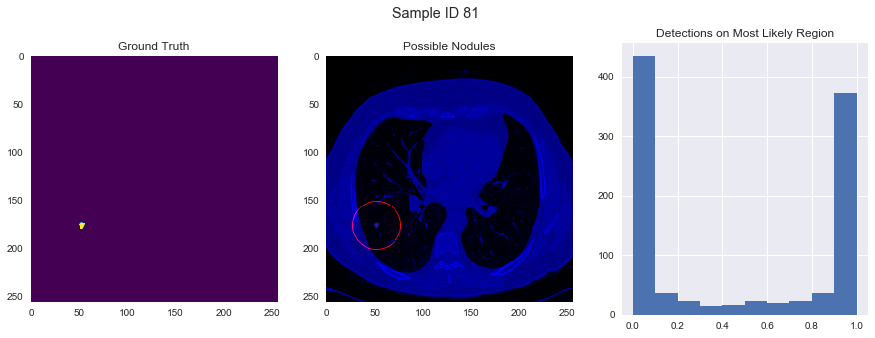
\includegraphics[scale=0.5]{conflicted_no_nodule.png} \\

As can be seen in the image, although the model probably would have classified the image as not having a lesion, we can see that the sample distribution in this case contributes significant information and might make a human expert to take a closer look into the image and perhaps what the model had missed. \\

In other cases, the sample distribution show no ambiguity about the classification. For example, we can see this behavior in the following cases: \\

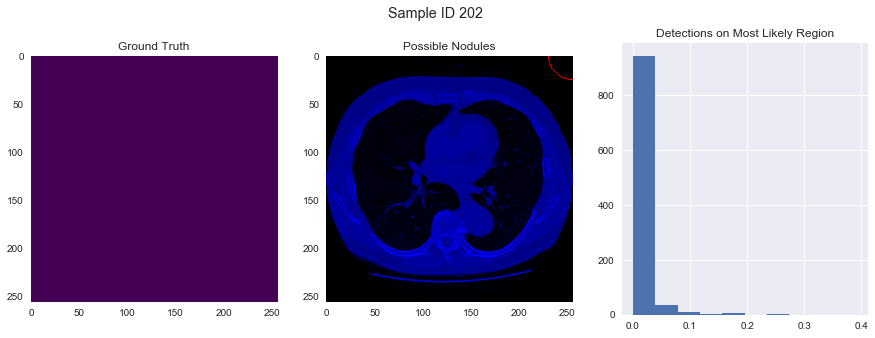
\includegraphics[scale=0.5]{Certain_no_nodule.png} \\

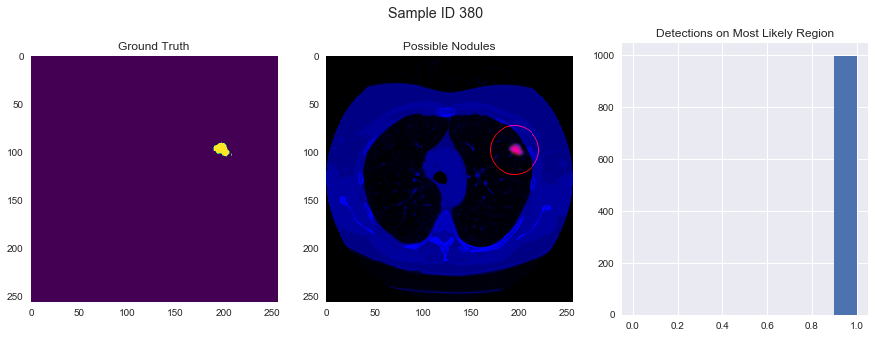
\includegraphics[scale=0.5]{sure_there_is_nodule.png} \\

In these cases the model shows certainty in the classification. This can also help a human expert to determine whether or not addition testing should be done to determine if a lesion is present. 

\subsubsection*{Hybrid Network}
The ROC curve shows that this model is not especially useful as a final diagnostic tool, and the posterior predictive distributions often show a very high level of uncertainty. The saliency maps do not show especially strong responses,  also indicating that the model is still unsure of how exactly to determine classification. We believe that the model may not be an optimal one for this task or the training regime needs to be modified for better performance. However, we are satisfied that our hybrid network and saliency maps visualization have offered us insight into why the model makes mistakes and performs poorly.

\subsection*{Conclusion and Future Work}
The use of Bayesian methods with deep learning models helps yield insights into the network's process and enhances the explainability of the model's predictions. The ability to localize and classify biomedical anomalies has the potential to improve the quality of patient care dramatically, and ultimately a patient's health outcome.

By assisting Radiologists with analyzing biomedical images, and giving them the ability to utilize the recolored images and the probability distributions generated from them, physicians can reach confident decisions more quickly. 

In the future, we would like to apply both the U-Net and Inception ResNet to the same dataset and analyze the results. Due to time constraints and data availability, we were unable to find a dataset that were viable for both approaches. With additional work, a single dataset could be engineered and be used to analyze how the networks can work together.

Additionally, expanding the U-Net to operate on 3D images rather than extract 2D slices would be highly beneficial. By extracting the 2-Dimensional slices, we lose the information that could be provided by the adjacent pixels in neighboring slices. Being able to take advantage of that additional information would likely improve the performance of U-Net segmentation.

\pagebreak
\subsection*{References}

\begin{enumerate}
\item\label{bib:baker} Baker, Darren, et al. \textit{Predicting Lung Cancer Incidence from CT Imagery}. Stanford University, 2017.

\item\label{bib:finale} Doshi-Velez, Finale, et al. ``Accountability of AI Under the Law: The Role of Explanation.'' \textit{SSRN Electronic Journal}, 2017, doi:10.2139/ssrn.3064761.

\item\label{ref:gal} Gal, Yarin, and Zoubin Ghahramani. \textit{Dropout as a Bayesian Approximation: Representing Model Uncertainty in Deep Learning}. University of Cambridge, 2016.

\item\label{bib:he} He, Kaiming, et al. ``Deep Residual Learning for Image Recognition.'' \textit{2016 IEEE Conference on Computer Vision and Pattern Recognition (CVPR)}, 2016, doi:10.1109/cvpr.2016.90.

\item\label{bib:ronneberger} Ronneberger, Olaf, et al. ``U-Net Convolutional Networks for Biomedical Image Segmentation.'' \textit{Informatik Aktuell Bildverarbeitung F??r Die Medizin}, 2017, doi:10.1007/978-3-662-54345.
\end{enumerate}


\end{document}